\documentclass[a4paper]{scrartcl}
\usepackage[utf8]{inputenc}
\usepackage[ngermanb]{babel}
\renewcommand{\familydefault}{\sfdefault}
\usepackage{ifpdf}
\usepackage{amsmath}
\usepackage{graphicx}
\usepackage{caption}
\title{MoHBF: Analytical Exercises IV: Signal Detection Theory}
\author{Stephan Gabler, 329231 \\ In cooperation with Rafael}

\date{\today}
\ifpdf
\fi
\begin{document}
\maketitle
\section{ROC Curves and PDFs}

The ROC curves can not uniquely determine the densities s(x) and n(x), because it is a plot of the integrals of the densities with respect to eachother. We loose information about the absolute location of the PDFs on the x-axis. Furthermore we do not know how the PDFs are scaled. And finally, if the PDFs do not overlap we also loose information of their relative position to eachother (the distance between the PDFs) and their shape. 

\begin{figure}[ht]
	\centering
		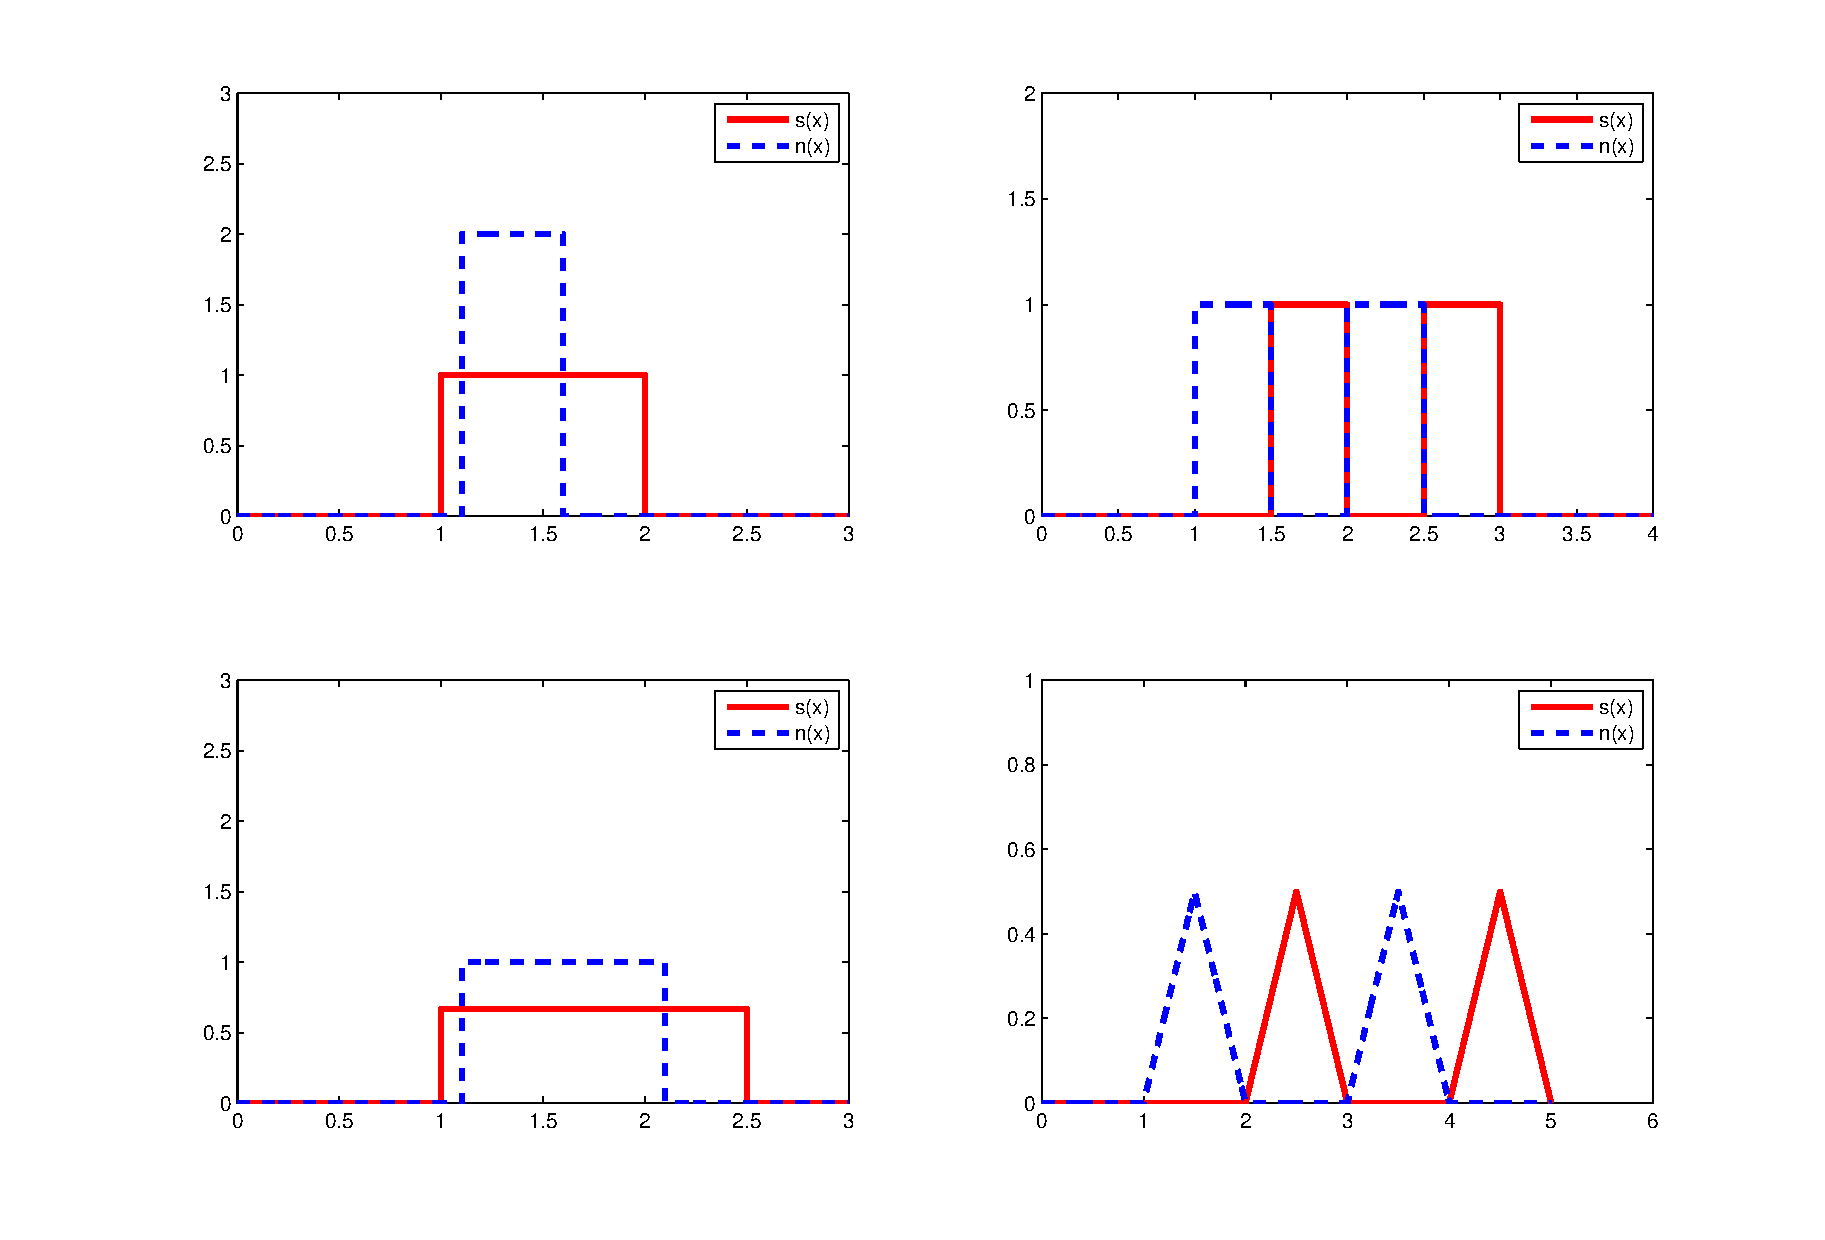
\includegraphics[width=0.7\textwidth]{pdfs.pdf}
			\caption{Two sets of densities s(x) and n(x) that could have resulted in the ROC curves shown on the assignment sheet. Left and right columns illustrate the probability distribution functions corresponding to the left and the right ROC curves, respectively.}
\label{sg:fig:pdfs}
\end{figure}

\clearpage

\section{Hits, False Alarms and the ROC Curve}

Integrals of the noise n(x) and the signal s(x) distributions:\\\\
\begin{equation}
	\int n(x)dx=\begin{cases}
	  {1\over 2}x,  & \text{for } -2 \leq x \leq 0\text{,}\\
	  0, & \text{else }
	\end{cases}\\\\\\
	\int s(x)dx=\begin{cases}
	  {1\over 2}(x+1)^2,  & \text{for } -1 \leq x < 0\text{,}\\
	  -{1\over 2}(1-x)^2,  & \text{for } 0 \leq x \leq 1\text{,}\\
	  0, & \text{else }
	\end{cases}\\\\
\end{equation}
False alarm rate p(FA) and hit rate p(H) for different values of $\lambda$:\\

\textbf{$\lambda = -3$:} \\

\begin{align*}
\int_{-2}^0n(x)dx &= -{1\over2}(-2) = 1 \mapsto p(FA) = 1.0 \\
\int_{-1}^0s(x)dx + \int_{0}^1s(x)dx &= 0.5 + 0.5 = 1\mapsto p(H) = 1.0
\end{align*}

\textbf{$\lambda = -1$:} \\

\begin{align*}
\int_{-1}^0n(x)dx &= -{1\over2}(-1) = 0.5 \mapsto p(FA) = 0.5 \\
\int_{-1}^0s(x)dx + \int_{0}^1s(x)dx &= 0.5 + 0.5 = 1\mapsto p(H) = 1.0
\end{align*}
\newpage
\textbf{$\lambda = -0.5$:} \\

\begin{align*}
\int_{-0.5}^0n(x)dx &= -{1\over2}(-0.5) = 0.25 \mapsto p(FA) = 0.25 \\
\int_{-0.5}^0s(x)dx + \int_{0}^1s(x)dx &= 1 - \int_{-1}^{-0.5}s(x)dx = 1 - 0.125 \mapsto p(H) = 0.875
\end{align*}

\textbf{$\lambda = {\sqrt{2}-2\over 2}$:} \\

\begin{align*}
\int_{{\sqrt{2}-2\over 2}}^0n(x)dx &\approx 0 - (-0.15) = 0.15 \mapsto p(FA) = 0.15  \\
\int_{\sqrt{2}-2\over 2}^0s(x)dx + \int_{0}^1s(x)dx &\approx 0.5 - 0.25 + 0.5 = 0.75 \mapsto p(H) = 0.75 
\end{align*}

\textbf{$\lambda = 0$:} \\

\begin{align*}
\int_{0}^\infty n(x)dx &= 0 \mapsto p(FA) = 0 \\
\int_{0}^1s(x)dx &= 0.5 \mapsto p(H) = 0.5
\end{align*}

\textbf{$\lambda = {2-\sqrt{2}\over 2}$:} \\

\begin{align*}
\int_{{2-\sqrt{2}\over 2}}^\infty n(x)dx &= 0 \mapsto p(FA) = 0 \\
\int_{2-\sqrt{2}\over 2}^1s(x)dx &\approx 0 - (-0.25) = 0.25 \mapsto p(H) = 0.25 
\end{align*}

\textbf{$\lambda = 0.5$:} \\

\begin{align*}
\int_{0.5}^\infty n(x)dx &= 0 \mapsto p(FA) = 0 \\
\int_{0.5}^1s(x)dx &= 0 - (-{1\over 8}) = 0.125 \mapsto p(H) = 0.125
\end{align*}

\textbf{$\lambda = 2$:} \\

\begin{align*}
\int_{2}^\infty n(x)dx &= 0 \mapsto p(FA) = 0 \\
\int_{2}^\infty s(x)dx &= 0 \mapsto p(H) = 0
\end{align*}

\begin{figure}[ht]
	\centering
		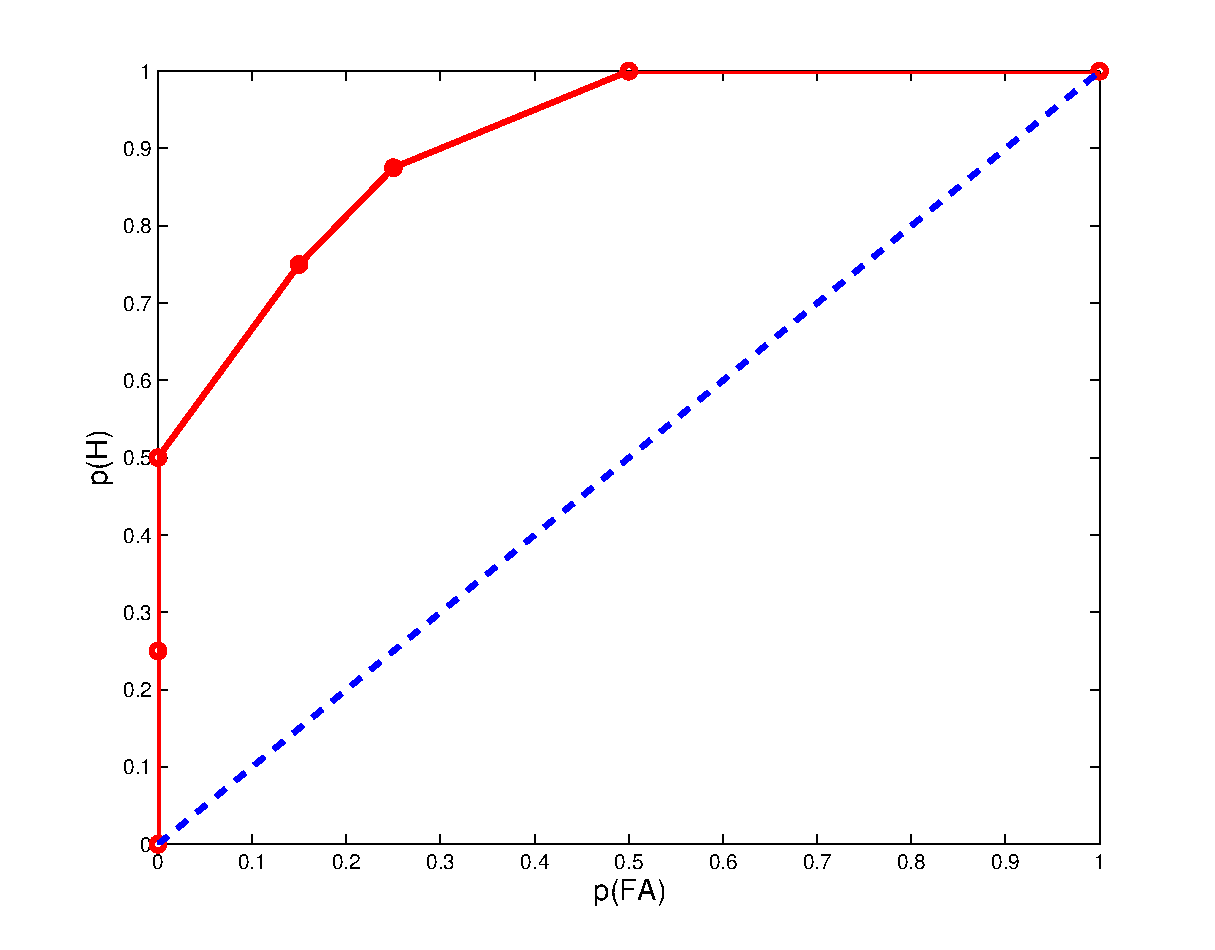
\includegraphics[width=0.8\textwidth]{roc.pdf}
	\caption{ROC curve computed from the PDFs illustrated on the assignment sheet using different values of $\lambda$ (see above).}
	\label{sg:fig:roc}
\end{figure}

\end{document}